
\begin{figure}[]
    \setlength{\resLen}{0.8in}
    %
    \centering
    \small
    \addtolength{\tabcolsep}{-5.5pt}
    %
    %
    \begin{tabular}{cccc}
        % &
        (a) \textbf{Ref} & (b) \textbf{Ours} & (c) \textbf{Relit1} & (d) \textbf{Relit2}
        \\ \vspace{-0.1em}
        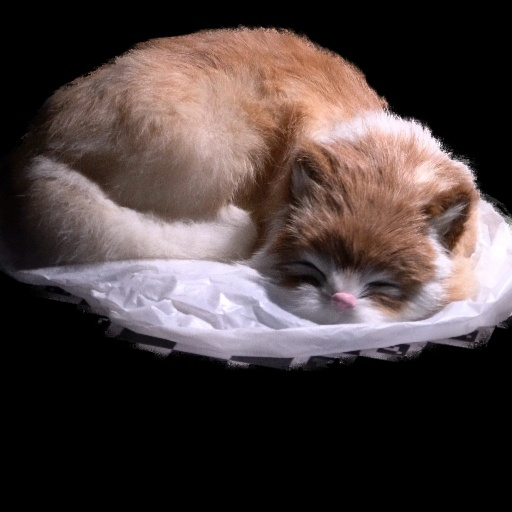
\includegraphics[trim={0pt 110pt 0pt 0pt},clip,width=\resLen]{images/relightable/cat/ref_orig.jpg} &
        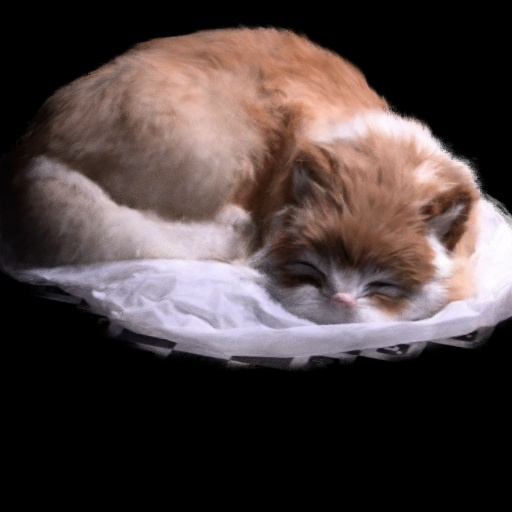
\includegraphics[trim={0pt 110pt 0pt 0pt},clip,width=\resLen]{images/relightable/cat/ours_orig.jpg} &
        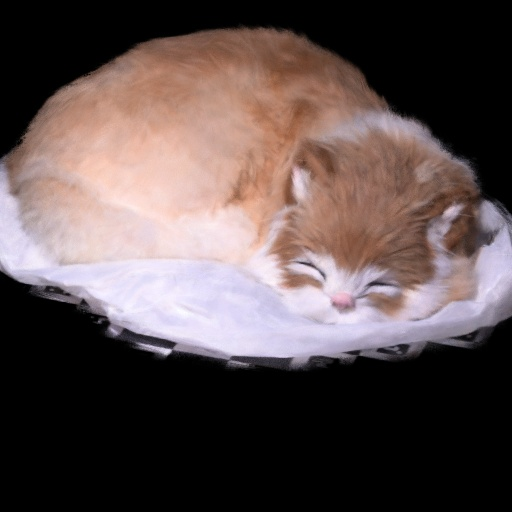
\includegraphics[trim={0pt 110pt 0pt 0pt},clip,width=\resLen]{images/relightable/cat/ours_relit1_.jpg} &
        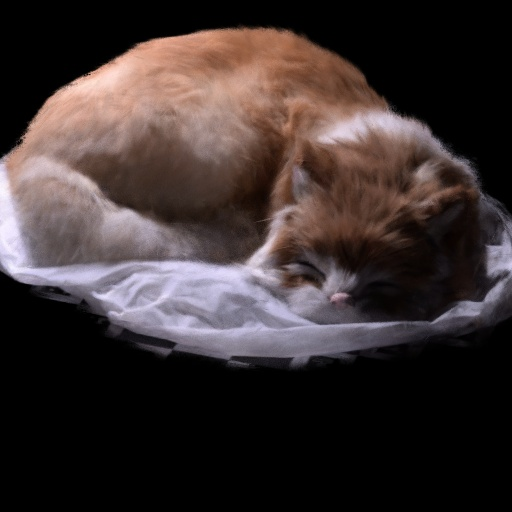
\includegraphics[trim={0pt 110pt 0pt 0pt},clip,width=\resLen]{images/relightable/cat/ours_relit2.jpg}
    \end{tabular}
    %
    \caption{
        Visualization of reconstruction and relighting for the \textit{Cat} scene. We show the reference (a), our reconstruction (b), and relighting under two novel lighting setups (c-d) not present in the training data.
    }
    \label{fig:rebuttal_relight}
\end{figure}